\documentclass[10pt]{exam}
\usepackage[hon]{template-for-exam}
\usepackage{endnotes,graphicx}
\usepackage{tikz,graphicx,enumitem,multicol,float,my-tikz-clipart,silence,cclicenses}
\graphicspath{{./figures/}}
\WarningFilter{latex}{Label `part}
\WarningFilter{latex}{There were multiply-defined labels}

\footer{}{\thepage}{\sc \myclass}


%\def\answer#1{\footnotetext{#1}}
%\def\myquestion{\item\stepcounter{footnote}}

\def\enoteheading{}
\def\answer#1{\endnotetext{#1}}
\def\theanswers{\theendnotes}
\def\myquestion{\item\stepcounter{endnote}}

\newenvironment{myquestions}{
  \begin{multicols}{2}\begin{enumerate}[resume]
}{
  \end{enumerate}\end{multicols}
}
\makeatletter
\patchcmd{\enit@setresumekeys}{\def}{\gdef}{}{}
\patchcmd{\enit@setresumekeys}{\def}{\gdef}{}{}
\makeatother

\newcommand{\myheading}[1]{\uplevel{\section*{#1}}
}
\newcommand{\mysubheading}[1]{\uplevel{\subsection*{#1}}
}

%uncomment if running Pandoc
% \renewcommand{\myheading}[1]{{\section*{#1}}}
% \renewcommand{\mysubheading}[1]{\subsection*{#1}}


\def\TestDay{Fri, May 8}


\def\mytitle{Chapters 20-21 HW (Circuits)}
\title{\mytitle}
\date{\today}

\def\mymaketitle{
  \begin{flushleft}
    {\LARGE \textbf \mytitle \par}
  \end{flushleft}
}

\newcommand{\bs}[2]{\textbf{#1} (\sc #2 Points)}


\newcommand{\GFig}[3]{  
  \begin{figure}[H]
    \centering
    \includegraphics[width=#3]{#1_#2_Figure.jpg}
    \caption{Giancolli Figure #1-#2.}
    \label{#1-#2}
  \end{figure}
}


\begin{document}
\maketitle
% \begin{center}
%   
\includegraphics[width=10cm]{sound-wave.png}
% \end{center}

\noindent
This HW is due on Mini-Test Day, \textbf{\TestDay}.

\vspace{1em}
\hrule

\vspace{1em}
\noindent
Questions and figures are from OpenStax \emph{College Physics}, 2e (Chapter 20-21) unless otherwise noted.


\section*{Ohm's Law Problems (Chapter 20)}

\begin{myquestions}

\myquestion (P2) \answer{333 mA}
  A total of 600~C of charge passes through a flashlight in 0.500~hr. What is the average current?

\myquestion (P18) \answer{0.833 A}
  What current flows through the bulb of a 3.00-V flashlight when its hot resistance is \SI{3.60}{\ohm}?
\columnbreak
\myquestion (P21) \answer{3.50 V}
  How many volts are supplied to operate an indicator light on a DVD player that has a resistance of \SI{140}{\ohm}, given that \SI{25.0}{mA} passes through it?
\end{myquestions}

\vs[6]

\section*{Circuits Concepts}


\begin{enumerate}[resume]
  
\myquestion (CQ2)
  Car batteries are rated in ampere-hours (\SI{}{A.h}). To what physical quantity do ampere-hours correspond (voltage, charge, current, resistance, etc), and what relationship do ampere-hours have to energy content?
  \vs 

\myquestion (Original Question)
  Is current directly proportional or inversely proportional to voltage?  Why does this make sense?
  \vs




\end{enumerate}

\pagebreak


\section*{Equivalent Resistance Problems (Chapter 21)}

\begin{myquestions}
\myquestion (P2) 
\answer{
  (a) \SI{6.60}{k\ohm}; 
  (b) $\frac{20}{213}\unit{k\ohm}=\SI{0.094}{k\ohm}$
}
  (a) What is the resistance of a 100-$\Omega$, a 2.50-k$\Omega$ , and a 4.00-k$\Omega$ resistor connected in series? (b) In parallel?

\myquestion (P3) \answer{\SI{786}{\ohm}; \SI{20.3}{\ohm}}
  What are the largest and smallest resistances you can obtain by connecting a 36.0-$\Omega$, a 50.0-$\Omega$, and a 700-$\Omega$ resistor together?

\myquestion (Original Problem) \answer{4.00 A}
  Find the current going through the battery in the circuit shown in Figure~\ref{circuit1}.
  %
  \begin{figure}[H]
    \centering
    
\includegraphics[width=5cm]{circuit1.pdf}
    \caption{Original Figure.}
    \label{circuit1}
  \end{figure}

\myquestion (Giancoli Ch 19 P16)
  Determine (a) the equivalent resistance of the circuit shown in Figure~\ref{19-48}, (b) thee voltage acros each resistor, and (c) the current through each resistor.
  %
  \begin{figure}[H]
    \centering
    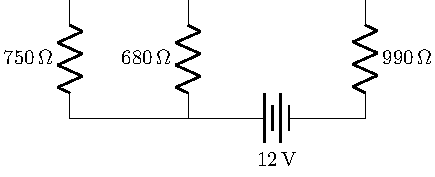
\includegraphics[width=6.5cm]{19_48_Figure.pdf}
    \caption{Giancolli Figure 19-48.}
    \label{19-48}
  \end{figure}


  \answer{ 
    Equivalent: $R = \SI{1346.6}{\ohm}$, $I = 8.9$ mA; \hfill
    \\\hspace*{2em} 990 \unit{\ohm}: $V = 8.8$ V,  $I = 8.9$ mA \hfill
    \\\hspace*{2em} 680 \unit{\ohm}: $V = 3.2$ V;  $I = 4.3$ mA \hfill
    \\\hspace*{2em} 750 \unit{\ohm}: $V = 3.2$ V;  $I = 4.7$ mA
  }
\end{myquestions}


\pagebreak

\section*{Equivalent Resistance Concepts}


\begin{enumerate}[resume]
  \myquestion (Original Question)
    What happens to resistance when bulbs are wired in series?  Why does this make sense? \vs
  
  \myquestion (Original Question)
    What happens to resistance when bulbs are wired in parallel?  Why does this make sense?
\end{enumerate}



\vs[2]

\hrule

\begin{myquestions}

\myheading{Additional Practice}

\myquestion (P1) \answer{(a) \SI{2750}{\ohm}; (b) \SI{27.5}{\ohm}}
  (a) What is the resistance of ten 275-$\Omega$  resistors connected in series? (b) In parallel?

\myquestion (Original Problem) \answer{1.36 A}
  Find the current going through the battery in the circuit shown in Figure~\ref{circuit2}.
  %
  \begin{figure}[H]
    \centering
    
\includegraphics[width=5cm]{circuit2.pdf}
    \caption{Original Figure.}
    \label{circuit2}
  \end{figure}

\columnbreak

\myheading{Bonus}


\myquestion
  Calculate the equivalent resistance of a cube that has a 1-ohm resistor along each edge, as shown in Figure~\ref{bonus-circuit},
  %
  \begin{figure}[H]
    \centering
    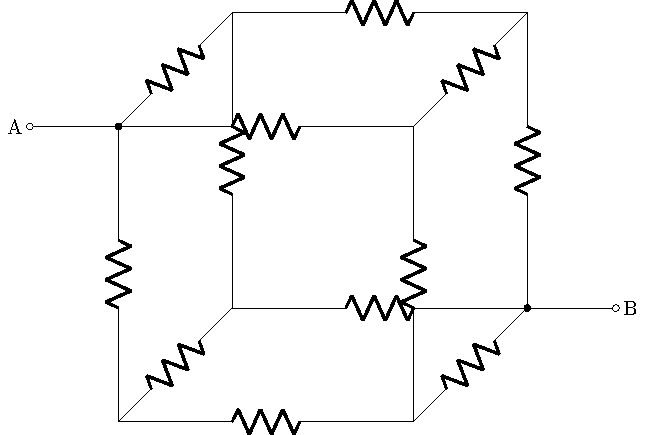
\includegraphics[width=6.5cm]{BonusCircuit.pdf}
    \caption{Original Figure.  Each resistor has a value of \SI{1}{\ohm}}
    \label{bonus-circuit}
  \end{figure}
  
\vspace*{\stretch{1}}


\end{myquestions}

\pagebreak


\section*{Equations}

\subsection*{Electrostatics Equations}

\begin{align*}
  F &= \frac{kq_1 q_2} {r^2} &
  E &\equiv \frac{F}{q} = \frac{kq}{r^2} &
  \Delta V &= -\frac{W}{q}
\end{align*}

\subsection*{Circuits Equations}

\begin{align*}
  I &\equiv \frac{\Delta q}{\Delta t} &
  \Delta V &= IR &
  P &= I\Delta V = I^2 R = \frac{\Delta V^2}{R}
\end{align*}


\begin{align*}
  R_{eq} &= R_1 + R_2 + \cdots &
  \frac{1}{R_{eq}} &= \frac{1}{R_1} + \frac{1}{R_2} + \vdots
\end{align*}

\subsection*{Unit Conversions}

\begin{align*}
  \SI{1}{mC} &= \SI{e-3}{C} &
  \SI{1}{\micro C} &= \SI{e-6}{C} &
  \SI{1}{n C} &= \SI{e-9}{C}
\end{align*}


\subsection*{Constants}

\vspace{2em}

\begin{tabular}{ll}
Coulomb Constant          &   $k = \SI{9.0e9}{\newton\meter^2\per\coulomb^2}$\\
Charge of electron/proton &   $e=\pm\SI{1.60e-19}{\coulomb}$\\
Electron mass             &   $m_e=\SI{9.11e-31}{\kilo\gram}$\\
Proton mass	              &   $m_p=\SI{1.673e-27}{\kilo\gram}$\\
Neutron mass	            &   $m_n=\SI{1.675e-27}{\kilo\gram}$
\end{tabular}

\vs
\hrule

\section*{Selected Answers}

  \renewcommand{\enotesize}{\normalsize}
  \renewcommand{\enoteformat}{%
    \leftskip=1.8em
    \makebox[0pt][r]{\theenmark. }%
  }

  \hfill

  \begin{multicols}{2}
    \theanswers
  \end{multicols}


\end{document}